\documentclass[presentation]{beamer}


\usepackage[utf8]{inputenc}
\usepackage[T1]{fontenc}
\usepackage{fixltx2e}
\usepackage{graphicx}
\usepackage{longtable}
\usepackage{float}
\usepackage{wrapfig}
\usepackage{rotating}
\usepackage[normalem]{ulem}
\usepackage{amsmath}
\usepackage{textcomp}
\usepackage{marvosym}
\usepackage{wasysym}
\usepackage{amssymb}
\usepackage{hyperref}
\tolerance=1000
\usepackage{graphicx}
\usepackage{tcolorbox}

\author{Laurent Gatto\\
University of Cambridge\\
\url{http://cpu.sysbiol.cam.ac.uk}}

\date{8 October 2014}

%% colors
\definecolor{Red}{rgb}{0.7,0,0}
\definecolor{Blue}{rgb}{0,0,0.8}

\usepackage{hyperref}
\usepackage{breakurl}
\hypersetup{%
  pdfauthor={Laurent Gatto},%
  pdfusetitle,
  bookmarks = {true},
  bookmarksnumbered = {true},
  bookmarksopen = {true},
  bookmarksopenlevel = 2,
  unicode = {true},
  breaklinks = {false},
  hyperindex = {true},
  colorlinks = {true},
  linktocpage = {true},
  plainpages = {false},
  linkcolor = {Blue},
  citecolor = {Blue},
  urlcolor = {Red},
  pdfstartview = {Fit},
  pdfpagemode = {UseOutlines},
  pdfview = {XYZ null null null}
}


\title{Computational Challenges in Mass Spectrometry-Based Spatial Proteomics}

\begin{document}

\maketitle


\begin{frame}
  \begin{figure}[h]
    \centering
    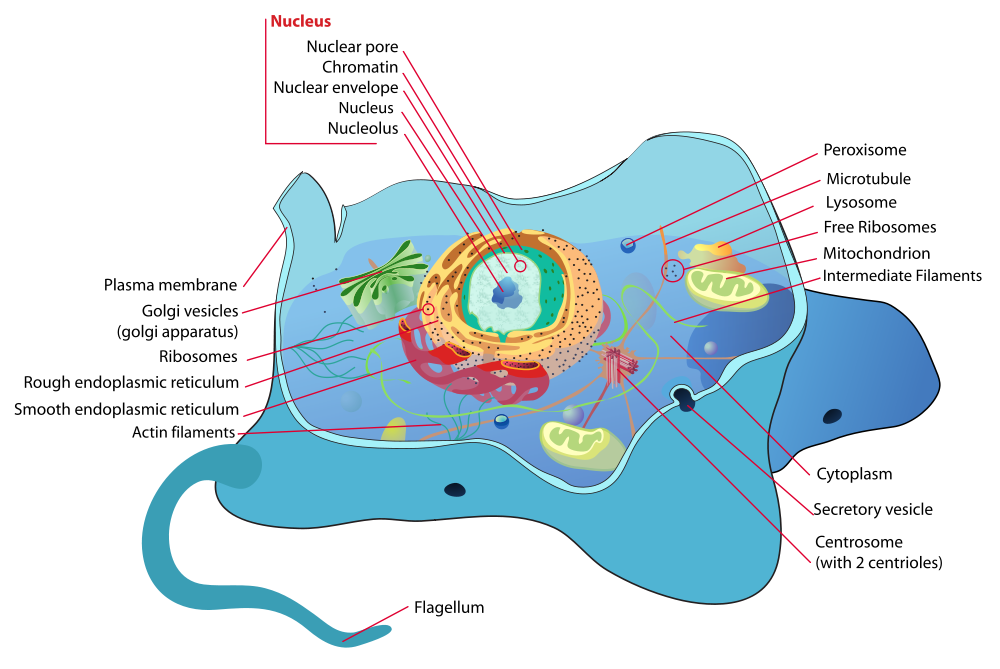
\includegraphics[width=.8\linewidth]{./figures/Animal_cell_structure.png}
  \end{figure}
\end{frame}

\begin{frame}
  \begin{figure}[h]
    \centering
    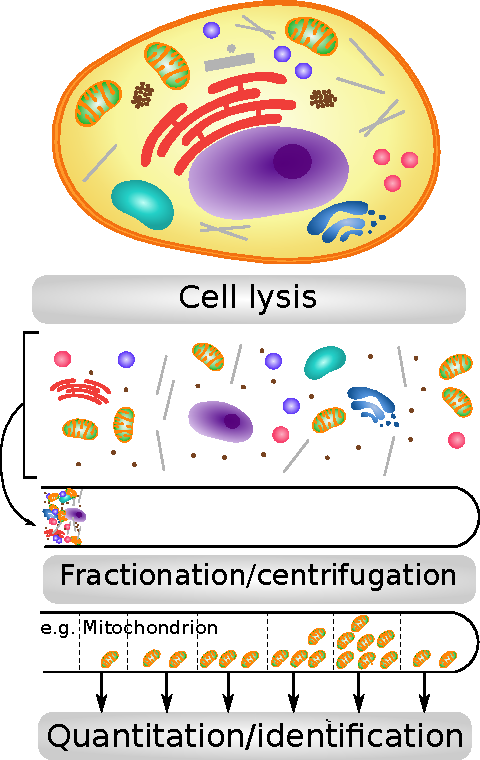
\includegraphics[width=.45\linewidth]{./figures/expdesign.pdf}
  \end{figure}
\end{frame}

\begin{frame}
  \begin{figure}[h]
    \centering
    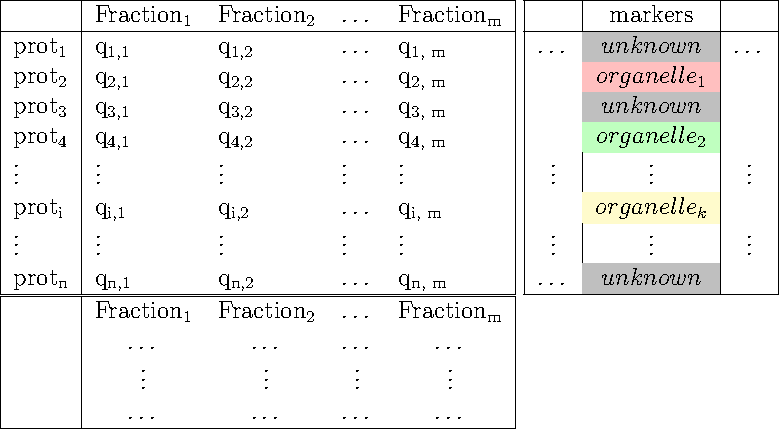
\includegraphics[width=.8\linewidth]{./figures/Fig1-data-a.pdf}
    \caption{Spatial proteomics data and metadata.}
  \end{figure}
\end{frame}

\begin{frame}
  \begin{figure}[h]
    \centering
    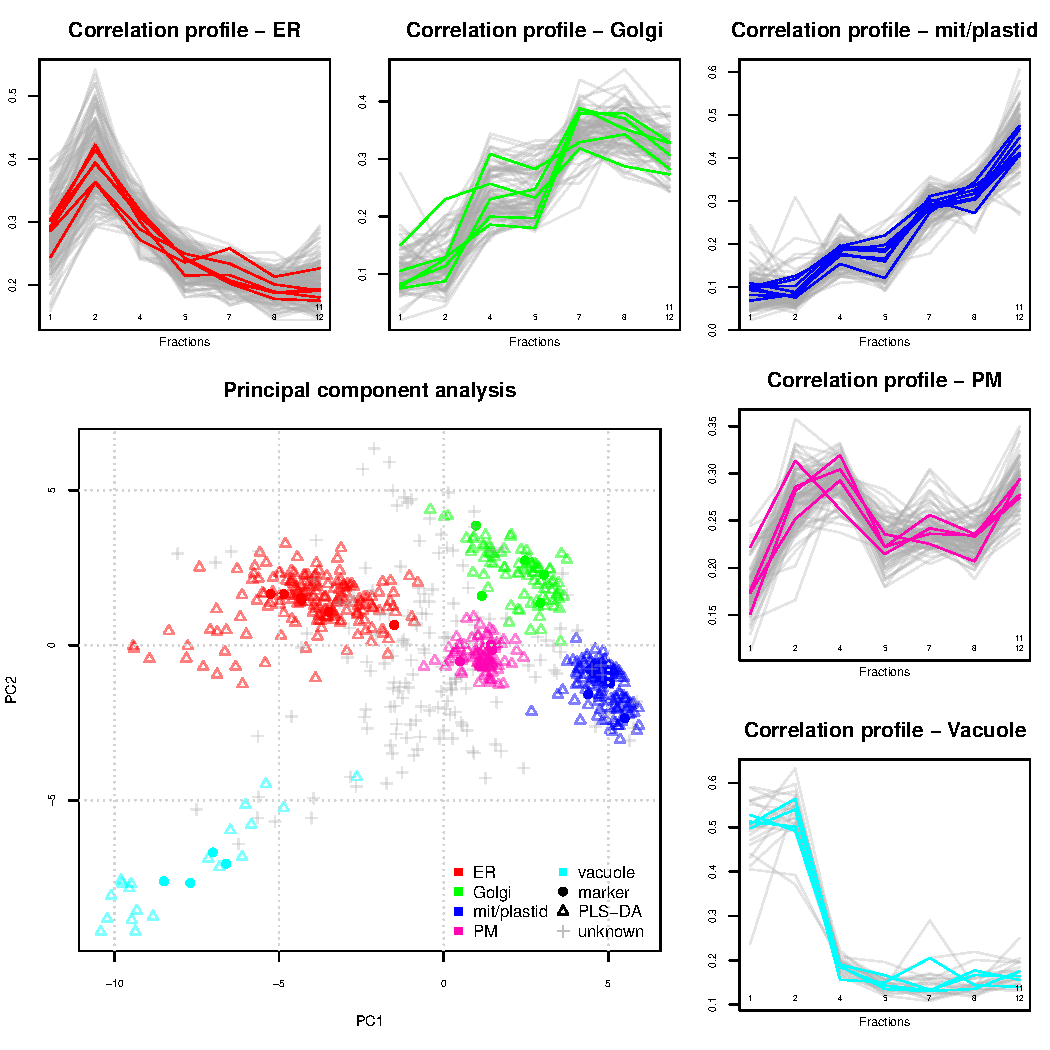
\includegraphics[width=.7\linewidth]{./figures/vis.pdf}
    \caption{Visualisation of protein profiles, Gatto \textit{et al.} (2010).}
  \end{figure}
\end{frame}


\begin{frame}{Challenge: resolution \textit{vs.} missing data}
  \begin{figure}[h]
    \centering
    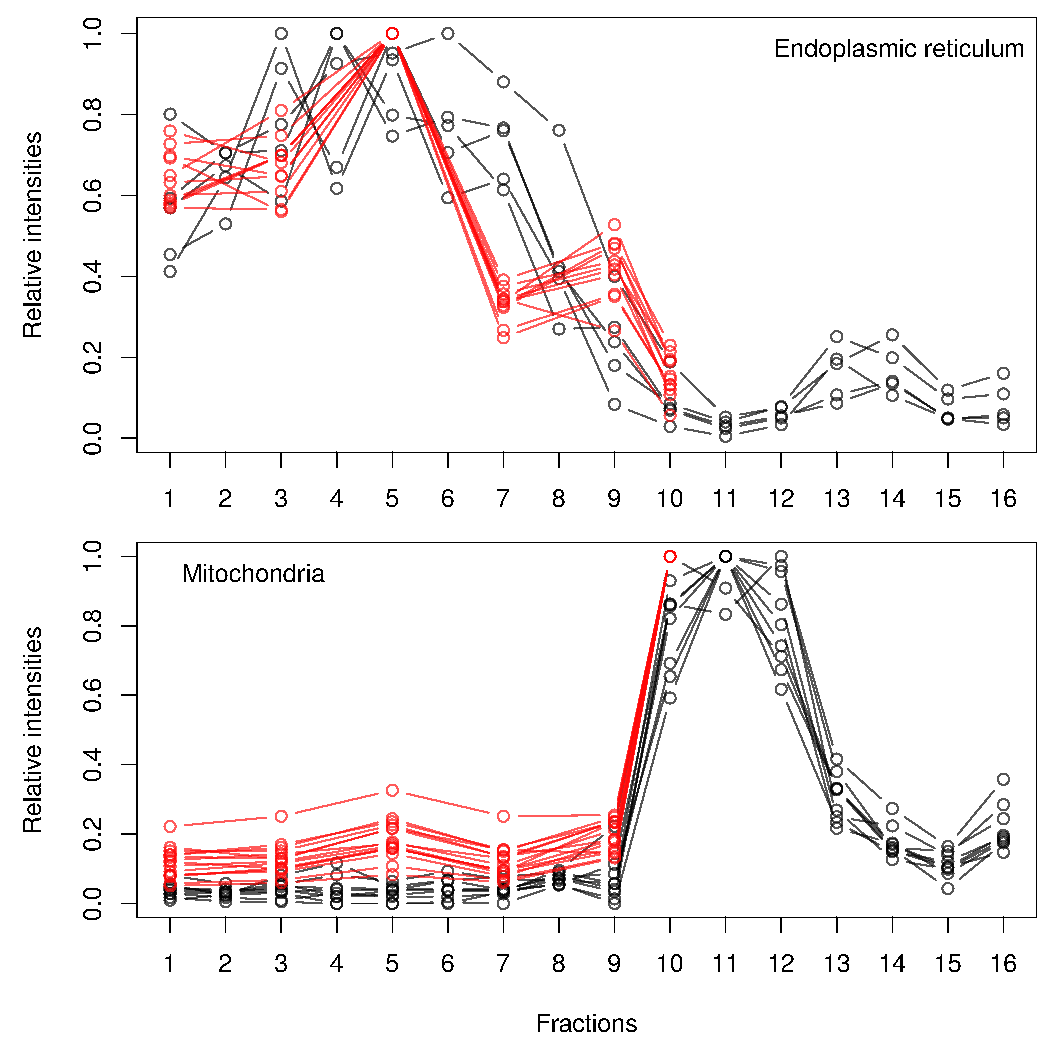
\includegraphics[width=.65\linewidth]{./figures/fractions.eps}
    \caption{More fractions of more proteins? Gatto \textit{et al.} (2014).}
  \end{figure}
\end{frame}

\begin{frame}{Challenge: resolution \textit{vs.} missing data}
  \begin{figure}[h]
    \centering
    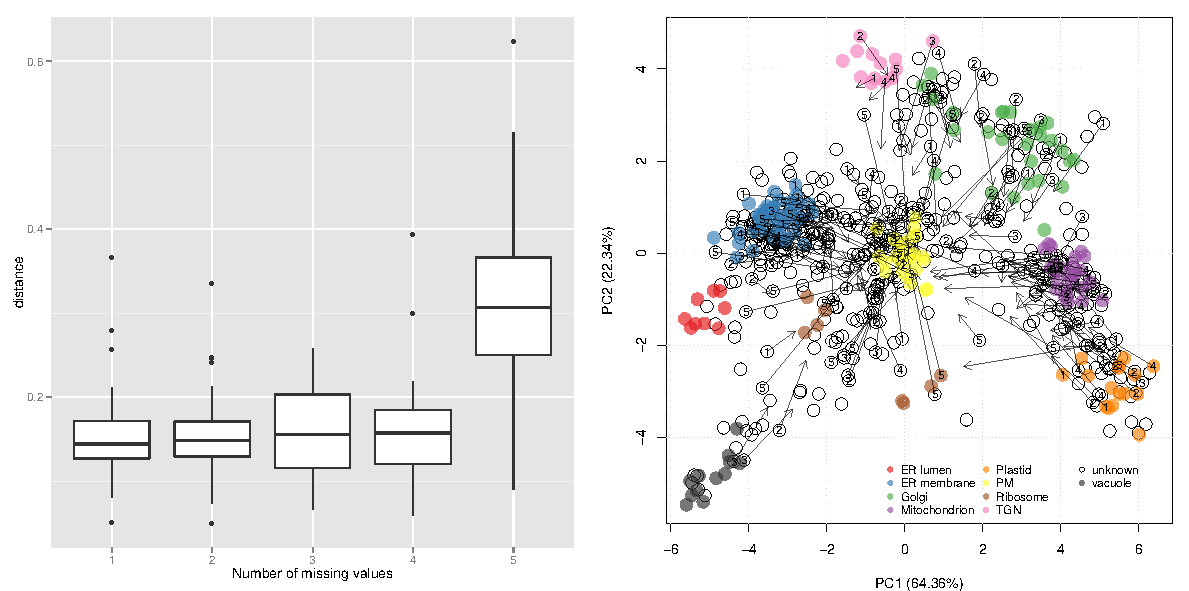
\includegraphics[width=.7\linewidth]{./figures/impute.pdf}
    \caption{Missing value imputation. Gatto \textit{et al.} (2014).}
  \end{figure}
\end{frame}

\begin{frame}{Challenge: spatial markers}
  \begin{figure}[h]
    \centering
    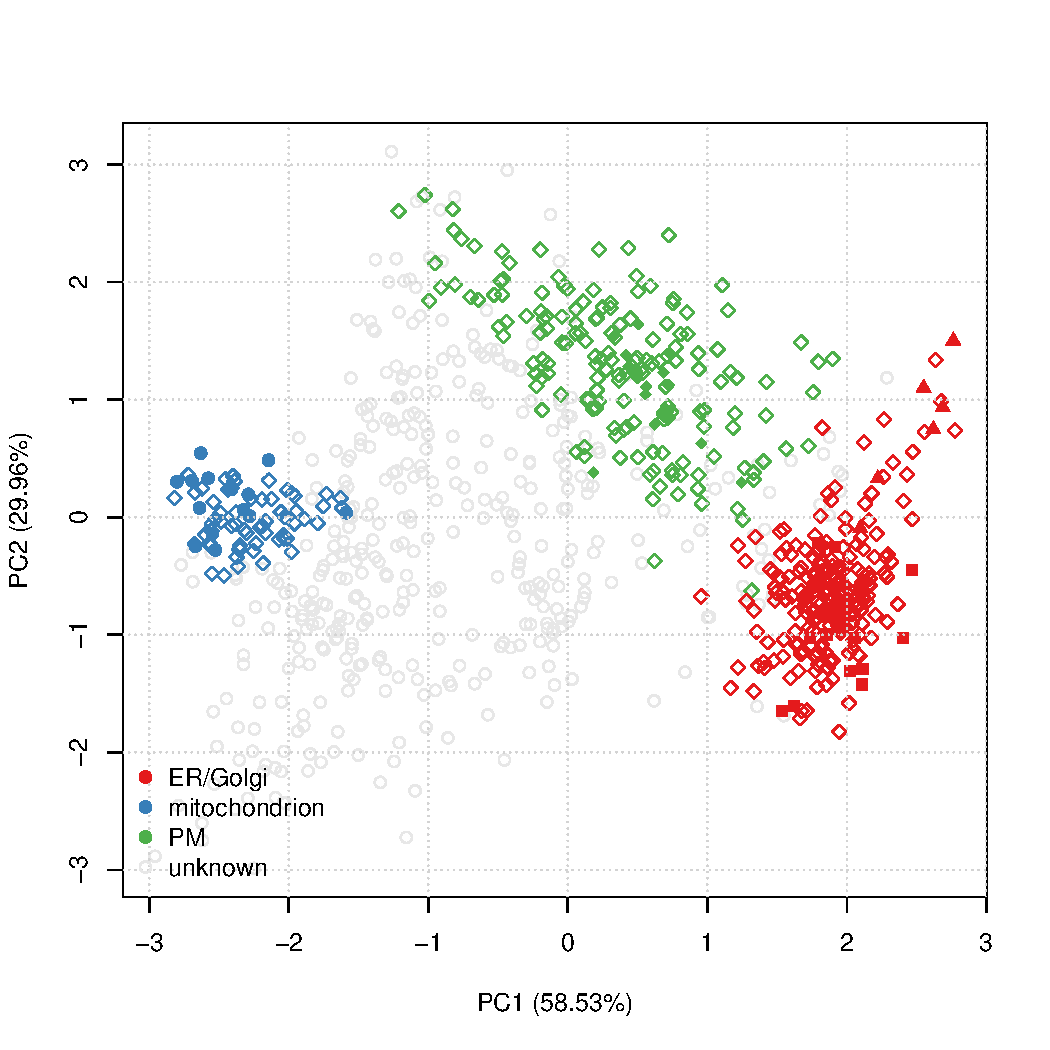
\includegraphics[width=.45\linewidth]{./figures/tan2009r1org.pdf}
    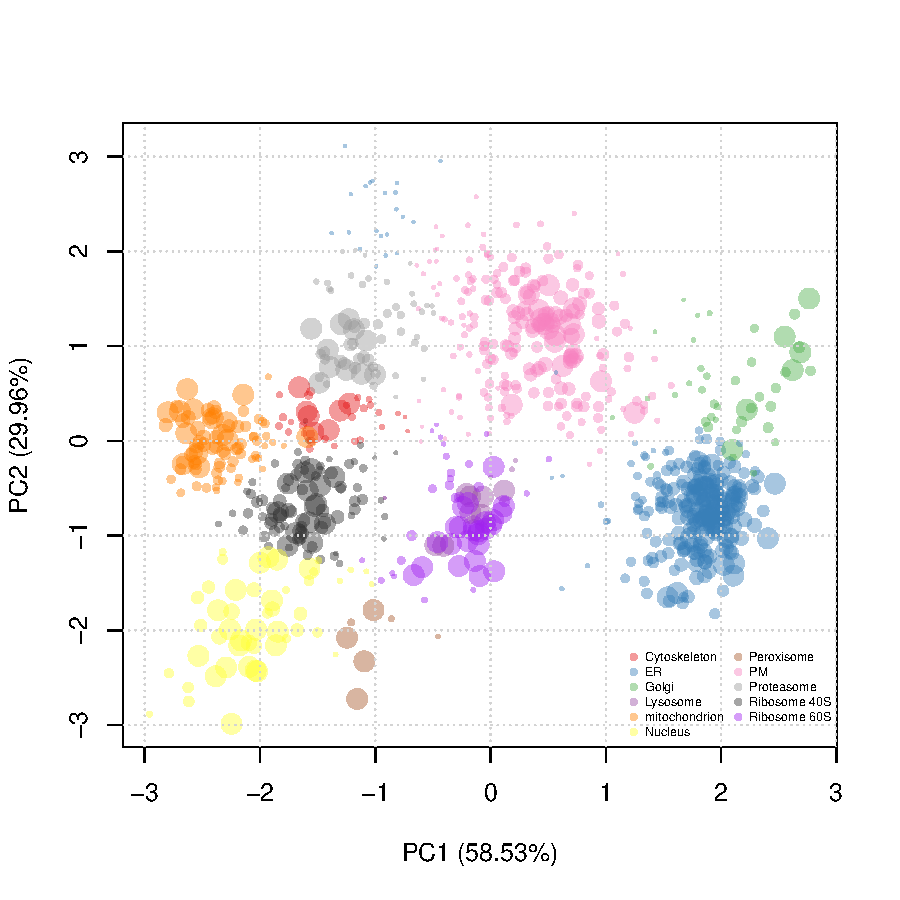
\includegraphics[width=.45\linewidth]{./figures/pdres2fig.pdf}
    \caption{Sub-cellular diversity. Tan \textit{et al.} (2009)
      vs. Breckels \textit{et al.} (2013). }
  \end{figure}
\end{frame}

\begin{frame}
  \begin{figure}[h]
    \centering
    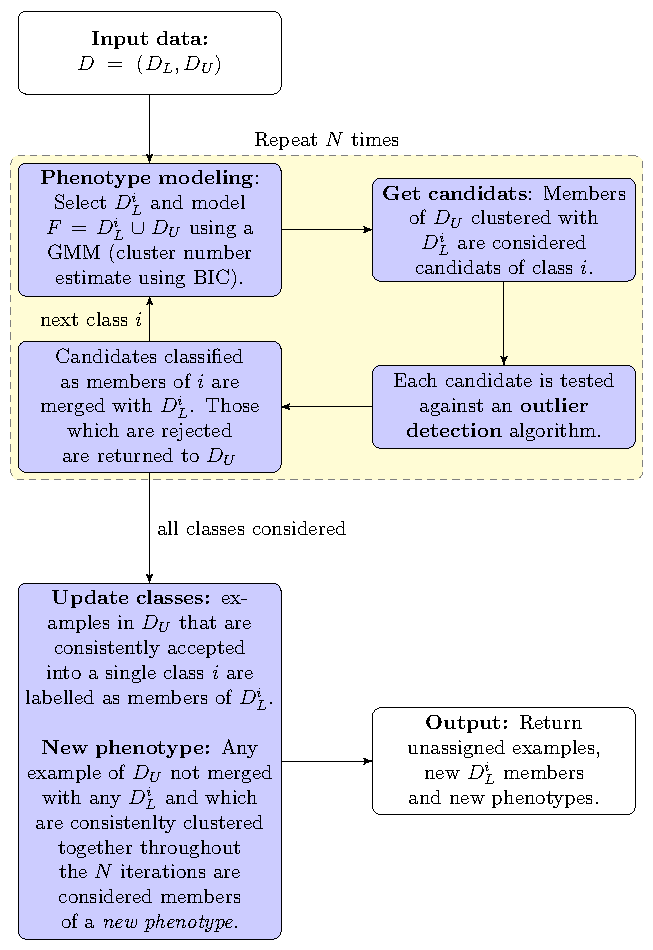
\includegraphics[width=.45\linewidth]{./figures/phenodisco.pdf}
  \end{figure}
\end{frame}


\begin{frame}{Challenge: spatial markers}
  \begin{figure}[h]
    \centering
    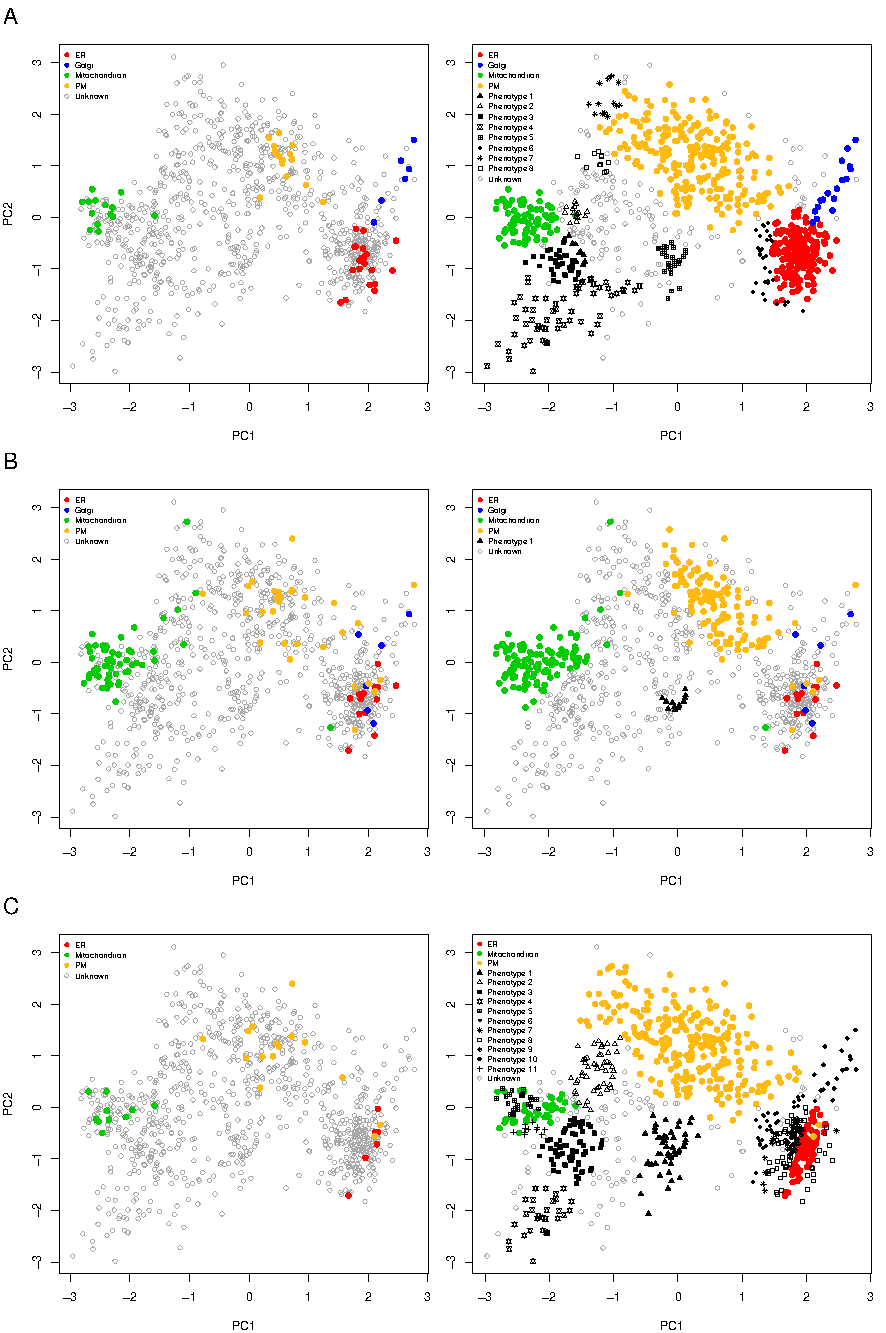
\includegraphics[width=.45\linewidth]{./figures/Fig6-pd.pdf}
    \caption{Quality of markers. Gatto \textit{et al.} (2014). }
  \end{figure}
\end{frame}


\begin{frame}{Challenge: dual localisation}
  \begin{figure}[h]
    \centering
    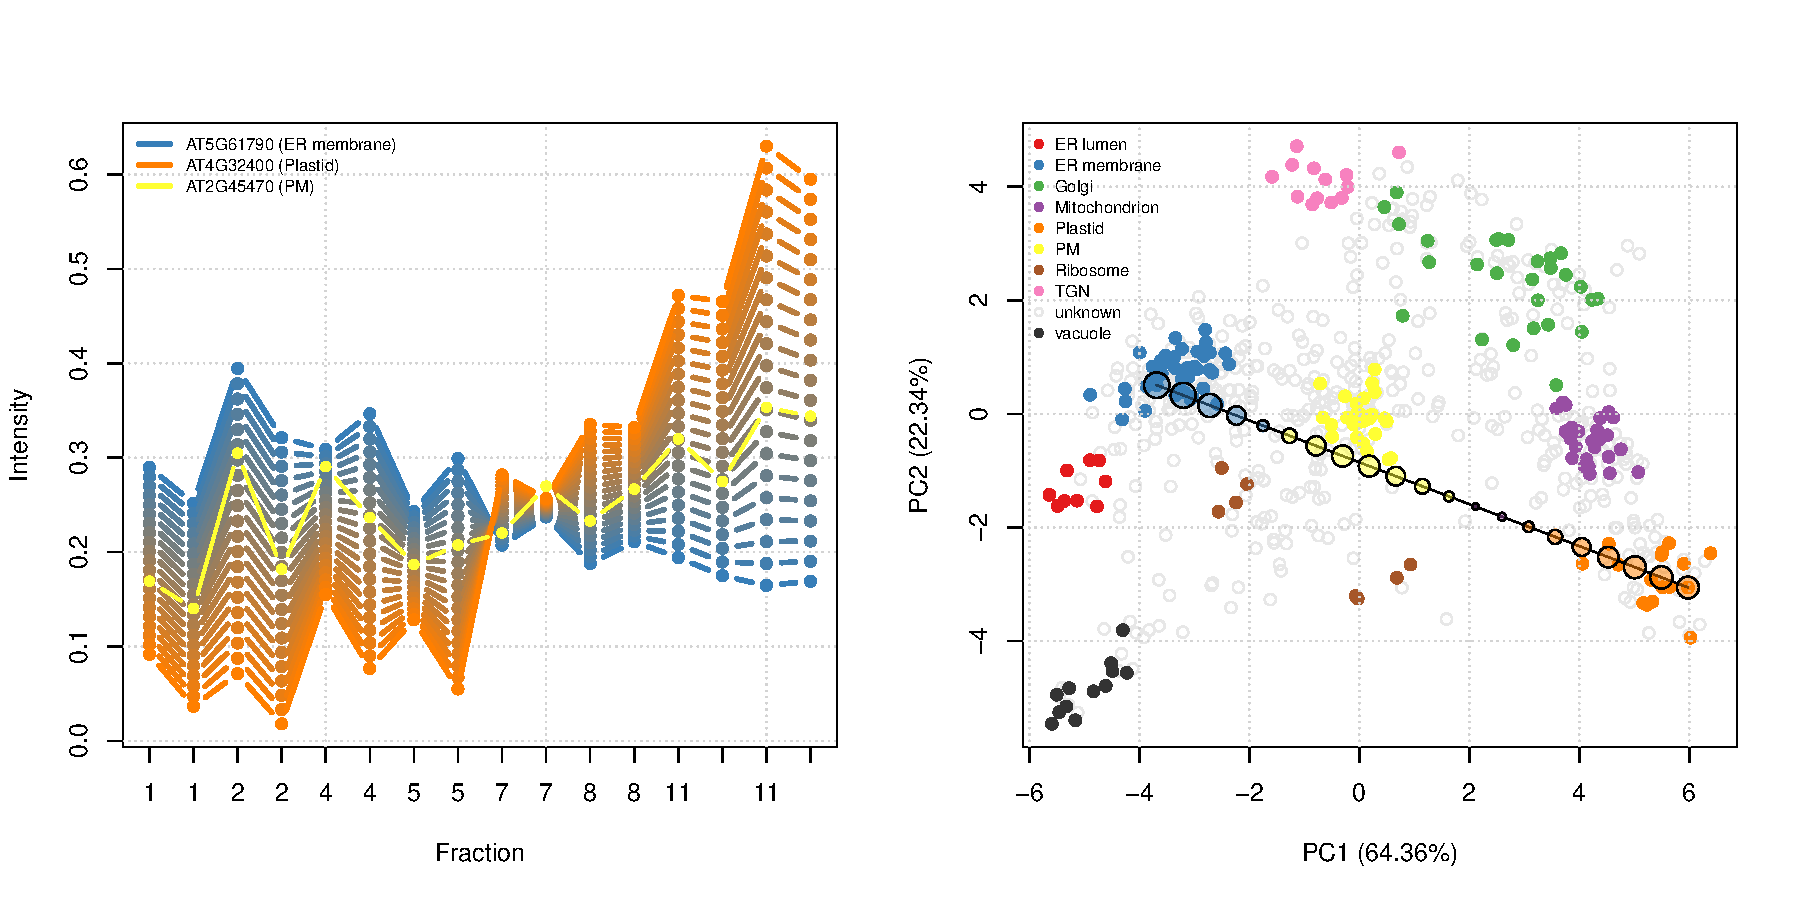
\includegraphics[width=.9\linewidth]{./figures/Fig-multiloc.pdf}
    \caption{Gatto \textit{et al.} (2014). }
  \end{figure}
\end{frame}

\begin{frame}{Challenge: dynamics}
  \begin{figure}[h]
    \centering
    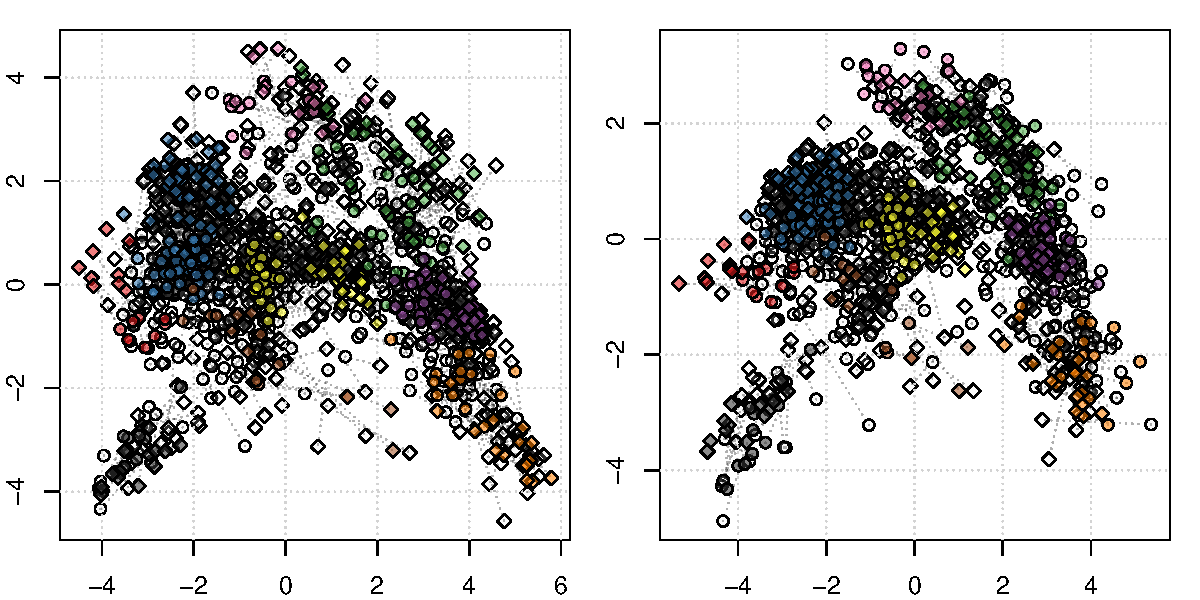
\includegraphics[width=.9\linewidth]{./figures/transloc-normalisation.pdf}
    \caption{Normalisation. Gatto \textit{et al.} (2014). }
  \end{figure}
\end{frame}

\begin{frame}{Challenge: dynamics}
  \begin{figure}[h]
    \centering
    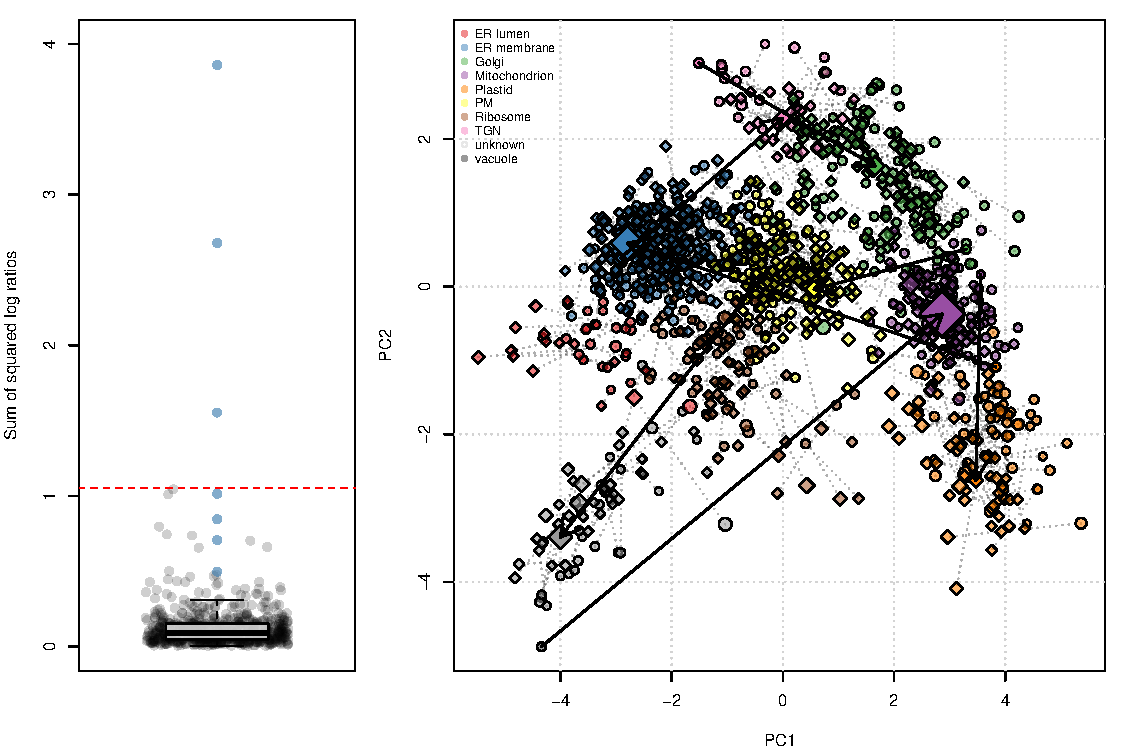
\includegraphics[width=.9\linewidth]{./figures/transloc-dynamics2.pdf}
    \caption{Statistics. Gatto \textit{et al.} (2014). }
  \end{figure}
\end{frame}
 
\begin{frame}{Conclusions}
  \begin{columns}
    \begin{column}<1->{.6\textwidth}
      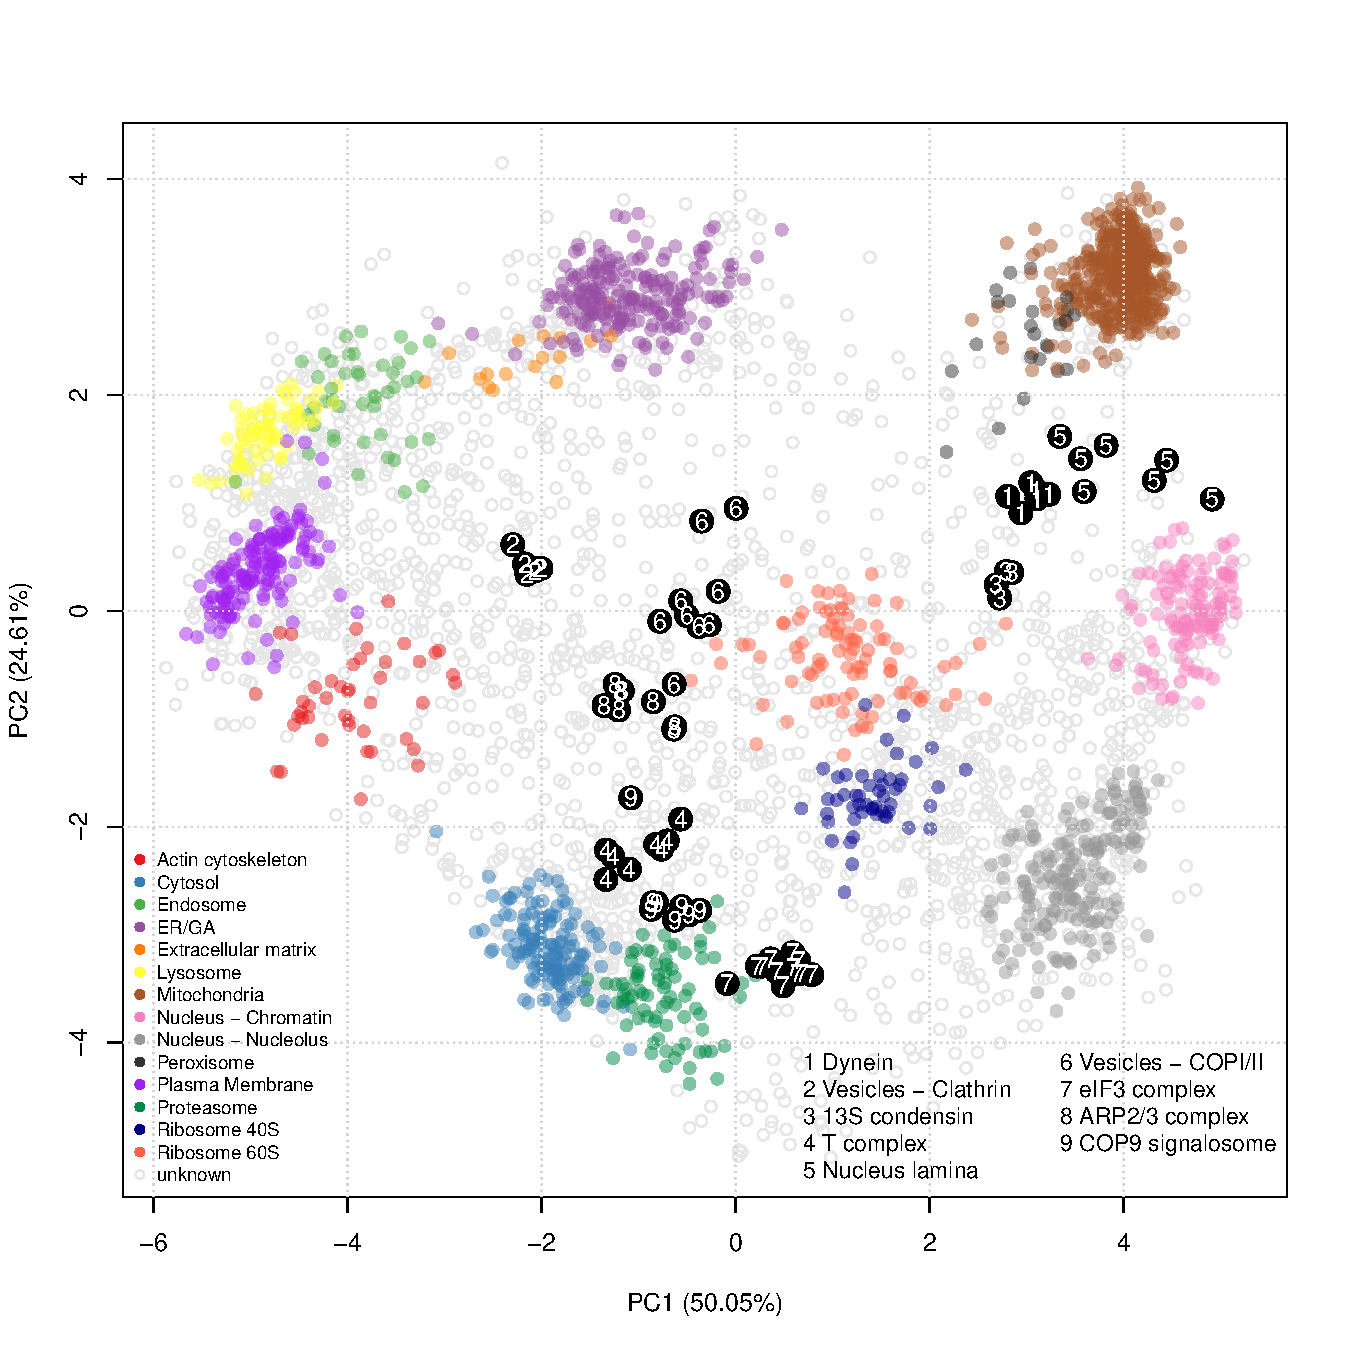
\includegraphics[width=1\linewidth]{./figures/fusfoi.pdf}
    \end{column}
    \begin{column}<2->{.4\textwidth}
      \begin{itemize}
      \item Mass spectrometry
      \item Experimental design
      \item Computational tools
      \end{itemize}
    \end{column}
  \end{columns}

\end{frame}


\begin{frame}
  \begin{itemize}
  \item Funding: BBSRC and FP7 Prime-XS
  \item Kathryn Lilley
  \item Lisa Breckels
  \end{itemize}

  \begin{tiny}
    
    \begin{thebibliography}{9}

    \bibitem{Gatto2010} Gatto L \textit{et al.}
      \emph{Organelle proteomics experimental designs and analysis.}
      Proteomics 2010 10(22):3957-69. PMID: 21080489.

    \bibitem{Breckels2013} Gatto L \textit{et al.}
      \emph{The effect of organelle discovery upon sub-cellular protein localisation.}
      J Proteomics 2013 88:129-40. PMMID 23523639.

    \bibitem{Gatto2014a} Gatto L \textit{et al.}
      \emph{A foundation for reliable spatial proteomics data analysis.}
      Mol Cell Proteomics 2014 13(8):1937-52. PMID: 24846987.

    \bibitem{Gatto2014b} Gatto L \textit{et al.}
      \emph{Mass-spectrometry-based spatial proteomics data analysis
        using {pRoloc} and {pRolocdata}.}  
      Bioinformatics 2014 30(9):1322-4. PMID: 24413670.

    \bibitem{prolocn} Gatto L \textit{et al.}
      \emph{A unifying bioinformatics framework for spatial proteomics.}  
      Bioconductor 2012 
      \url{http://www.bioconductor.org/package/release/bioc/html/pRoloc.html}

    \end{thebibliography}

  \end{tiny}

\end{frame}

\end{document}